\documentclass[cs4size,a4paper]{ctexart}   
%==================== 数学符号公式 ============
\usepackage{caption}
\usepackage{subfigure}
\usepackage[algo2e,ruled,vlined,linesnumbered]{algorithm2e} % 伪代码包
\usepackage{enumerate}
\usepackage{amsmath}                 % AMS LaTeX宏包
\usepackage[style=1]{mdframed}
\usepackage{amsthm}
\usepackage{amsfonts}
\usepackage{mathrsfs}                % 英文花体字 体
\usepackage{bm}                      % 数学公式中的黑斜体
\usepackage{bbding,manfnt}           % 一些图标,如 \dbend
\usepackage{lettrine}                % 首字下沉,命令\lettrine
\def\attention{\lettrine[lines=2,lraise=0,nindent=0em]{\large\textdbend\hspace{1mm}}{}}
\usepackage{longtable}
\usepackage[toc,page]{appendix}
\usepackage{geometry}                % 页边距调整
\geometry{top=3.0cm,bottom=2.7cm,left=2.5cm,right=2.5cm}
%====================公式按章编号==========================
\numberwithin{equation}{section}
\numberwithin{table}{section}
\numberwithin{figure}{section}
%================= 基本格式预置 ===========================
\usepackage{fancyhdr}
\pagestyle{fancy}
\fancyhf{}  
\fancyhead[C]{\zihao{5}  \kaishu 机\ 器\ 学\ 习\ 结\ 课\ 报\ 告}
\fancyfoot[C]{~\zihao{5} \thepage~}
\renewcommand{\headrulewidth}{0.65pt} 
%\CTEXsetup[format={\centering\bfseries\zihao{-2}}]{section}
\ctexset{
    section={format={\centering\bfseries\zihao{-2}}},
    subsection={nameformat={\bfseries\zihao{3}}},
    subsubsection={nameformat={\bfseries\zihao{4}}}
}
\setcounter{tocdepth}{2}             % 设置目录 
%================== 图形支持宏包 =========================
\usepackage{subfigure}
\usepackage{graphicx}                % 嵌入png图像
\usepackage{color,xcolor}            % 支持彩色文本、底色、文本框等
\usepackage{svg-extract}
\usepackage{hyperref}                % 交叉引用
\usepackage{caption}
\captionsetup{figurewithin=section}
%==================== 源码和流程图 =====================
\usepackage{listings}                % 粘贴源代码
\usepackage{xcolor}
\usepackage{color}
\definecolor{dkgreen}{rgb}{0,0.6,0}
\definecolor{gray}{rgb}{0.5,0.5,0.5}
\definecolor{mauve}{rgb}{0.58,0,0.82}
\usepackage{xcolor}
\lstset{
    %行号
    numbers=left,
    %背景框
    framexleftmargin=8mm,
    frame=none,
    %背景色
    %backgroundcolor=\color[rgb]{1,1,0.76},
    backgroundcolor=\color[RGB]{245,245,244},
    %样式
    keywordstyle=\bf\color{blue},
    identifierstyle=\bf,
    numberstyle=\color[RGB]{0,192,192},
    commentstyle=\it\color[RGB]{0,96,96},
    stringstyle=\rmfamily\slshape\color[RGB]{128,0,0},
    %显示空格
    showstringspaces=false
}


%--------------------
\hypersetup{hidelinks}
\usepackage{booktabs}  
\usepackage{tabularx}
\usepackage{shorttoc}
\usepackage{tabu,tikz}
\usepackage{float}

\usepackage{multirow}



\tabcolsep=1ex
\tabulinesep=\tabcolsep
\newlength\tikzboxwidth
\newlength\tikzboxheight
\newcommand\tikzbox[1]{
    \settowidth\tikzboxwidth{#1}
    \settoheight\tikzboxheight{#1}
    \begin{tikzpicture}
        \path[use as bounding box]
            (-0.5\tikzboxwidth,-0.5\tikzboxheight)rectangle
            (0.5\tikzboxwidth,0.5\tikzboxheight);
        \node[inner sep=\tabcolsep+0.5\arrayrulewidth,line width=0.5mm,draw=black]
            at(0,0){#1};
    \end{tikzpicture}%
}

\makeatletter
\def\hlinew#1{
    \noalign{\ifnum0=`}\fi\hrule \@height #1 \futurelet
    \reserved@a\@xhline
}
   
\newcommand{\tabincell}[2]{\begin{tabular}{@{}#1@{}}#2\end{tabular}}%

\usepackage{subfigure}

\usepackage{ifthen}


\usepackage{graphicx} 
\newcommand{\HRule}{\rule{\linewidth}{0.5mm}}

\newtheorem{Theorem}{定理}
\newtheorem{Lemma}{引理} 
%%使得公式随章节自动编号
\makeatletter
\@addtoreset{equation}{section}
\makeatother
\renewcommand{\theequation}{\arabic{section}.\arabic{equation}}

%-------------------------
	
\usepackage{pythonhighlight}
\usepackage{tikz}                    
\usepackage{tikz-3dplot}
\usetikzlibrary{shapes,arrows,positioning}
%===================   正文开始    ===================
\begin{document}
% \bibliographystyle{gbt7714-2005}     %论文引用格式
%===================  定理类环境定义 ===================
\newtheorem{example}{例}              % 整体编号
\newtheorem{algorithm}{算法}
\newtheorem{theorem}{定理}            % 按 section 编号
\newtheorem{definition}{定义}
\newtheorem{axiom}{公理}
\newtheorem{property}{性质}
\newtheorem{proposition}{命题}
\newtheorem{lemma}{引理}
\newtheorem{corollary}{推论}
\newtheorem{remark}{注解}
\newtheorem{condition}{条件}
\newtheorem{conclusion}{结论}
\newtheorem{assumption}{假设}
%==================重定义 ===================
\renewcommand{\contentsname}{目录}     
\renewcommand{\abstractname}{摘要} 
\renewcommand{\refname}{参考文献}     
\renewcommand{\indexname}{索引}
\renewcommand{\figurename}{图}
\renewcommand{\tablename}{表}
\renewcommand{\appendixname}{附录}
\renewcommand{\proofname}{证明}
\renewcommand{\algorithm}{算法} 
%============== 封皮和前言 =================
\begin{titlepage}

\begin{center}


% Upper part of the page
 

{\huge \bfseries 华中科技大学计算机科学与技术学院}\\[1.5cm]

{ \huge \bfseries 《机器学习》结课报告}\\[1.5cm]


\includegraphics[width=0.55\textwidth]{figure/logo1.png}\\[1.5cm]   



% Title


% Author and supervisor

\begin{minipage}{0.5\textwidth}
\large
{\heiti 专~~~~~~~业}\quad \underline{~计算机科学与技术~} 

{\heiti 班~~~~~~~级}\quad \underline{~~~~~~~~~CS2203~~~~~~~~~}

{\heiti 学~~~~~~~号}\quad \underline{~~~~~~U202215634~~~~~~}

{\heiti 姓~~~~~~~名}\quad \underline{~~~~~~~~~黄君翊~~~~~~~~~}

{\heiti 成~~~~~~~绩}\quad \underline{~~~~~~~~~~~~~~~~~~~~~~~~~~~~}

{\heiti 指导教师}\quad \underline{~~~~~~~~~张~~~~腾~~~~~~~~~}

{\heiti 时~~~~~~~间}\quad \underline{~\today~}
\end{minipage}

\vfill

\end{center}

\end{titlepage}

\pagestyle{plain}
\pagenumbering{Roman}
\pagestyle{empty}
\tableofcontents 
\thispagestyle{empty}
%============== 论文正文   =================
\pagestyle{fancy}
\pagenumbering{arabic}
\setlength{\headheight}{12.64723pt}
\addtolength{\topmargin}{-0.64723pt}
\section{实验要求}

总体要求:

\begin{enumerate}
    \item 控制报告页数,不要大段大段贴代码
    \item 表格和插图请编号并进行交叉引用,表格使用三线表
\end{enumerate}







\section{算法设计与实现}

本次实验我选择参考选题四:数字识别,数据集为MNIST手写数字数据集,模型使用CNN卷积神经网络(基于numpy实现)\cite{zhouzhihua},对test.csv预测上传kaggle,并与pytorch现有模型进行对比。

\subsection{算法目标}

使用numpy从零开始搭建CNN卷积神经网络,实现其中的全连接层、卷积层、池化层等的正向和反向传播,并以此搭建Lenet-5网络进行小批量随机梯度下降(SGD)训练,验证Lenet-5在MNIST数据集上的效果,另外与KNN对比,并在测试集上达到一定准确度,最终解决手写数字识别问题,最后将实现代码上传github。

\subsection{数据集分析和处理}

使用pandas库读取train.csv并分析数据集构成。数据集共785个列,第一列为label,后784列为单通道28*28的灰度图片,取值$[0, 255)$的整数,使用matplotlib读取前9张图片,如图\ref{fig2-1}

\begin{figure}[h!]
    \centering
    \includesvg[width=0.7\textwidth]{figure/train-9}
    \caption{可视化训练集}
    \label{fig2-1}
\end{figure}

此时的数据并不能直接用来训练,模型只接受numpy支持的数组ndarray,首先我们需要将dataframe转换为ndarray,然后将label和feature分离,取出第一列作为train\_label,剩下的reshape到28*28的矩阵后作为train\_feature。

之后我们还需要从训练集中划分一部分作为验证集来在训练中实时检测模型的准确率,使用sklearn包中的train\_test\_split来进行数据集的随机划分,我的实现取了80\%的数据用于训练,剩下的用于验证。

CNN网络训练需要大量样本,为了加速训练,也保证训练集的随机性,我们需要将数据集划分为小批量(batch)进行处理,在这里我使用pytorch包中的DataLoader来加载数据,每一次取出128个数据作为(128, 1, 28, 28)(批量大小,通道,高,宽)的tensor张量,(按照实验要求)转换为ndarray后训练,数据类型设置为np.float64(后期发现代码中还有一部分是np.float32,没有完全改过来)。

最后,得到的训练样本每一个像素取值在0到255之间,为了加速模型收敛,减小数据尺度,防止梯度爆炸和数据溢出的问题,将像素值除以256进行归一化。

\subsection{神经网络层实现}

卷积神经网络(CNN)是一种深度学习模型\cite{o2015introduction},广泛应用于图像分类、目标检测、图像分割、图像生成、视频分析以及自然语言处理等领域。在这里为了能够搭建一个CNN网络,首先需要实现其基本组件:卷积层、池化层、全连接层等。

\subsubsection{卷积层}

卷积层(Convolution)是CNN的核心组件,在图像处理和特征提取中起着至关重要的作用。卷积层不一次性处理整个图像,而是通过一个卷积核逐步扫描图像的局部区域,自动学习和提取最有用的特征。一张图像共享一个卷积核的参数,参数共享大大减少了模型的参数数量,相比全连接层,是一种稀疏连接的层。

前向传播中,具体的计算过程,卷积层包含in\_channel, out\_channel, padding, stride, bias五个参数,前两个确定图片输入的通道数和最后输出的通道数,padding决定是否需要对图片四周向外填充数据,stride决定卷积核扫描的步幅,bias决定该卷积层是否需要偏置。设输入数据维度为 $(N, C_{in}, H_{in}, W_{in})$,其中 $N$ 是批大小(batch size),$C_{in}$ 是输入通道数,$H_{in}$ 和 $W_{in}$ 分别是输入的高度和宽度,带偏置。那么卷积核的维度为 $(C_{out}, C_{in}, K_h, K_w)$,其中 $C_{out}$ 是输出通道数,$K_h$ 和 $K_w$ 分别是卷积核的高度和宽度。卷积操作的输出维度为 $(N, C_{out}, H_{out}, W_{out})$,其中:
\[
H_{out} = \left\lfloor \frac{H_{in} - K_h + 2P}{S} \right\rfloor + 1
\]
\[
W_{out} = \left\lfloor \frac{W_{in} - K_w + 2P}{S} \right\rfloor + 1
\]
$P$ 是padding大小,$S$ 是步幅stride,常用的情况:卷积核长宽都为3,padding为1,stride为1时,保持图片原大小不变。

高维度下卷积公式晦涩难懂,对于每一个输入通道和输出通道对应一个卷积核,类似全连接层。设卷积核权重$W$,偏置$b$这一组卷积的前向传播公式如下:

\[
Y_{h,w} = \sum_{i=0}^{K_h-1} \sum_{j=0}^{K_w-1} X_{h+i, w+j} \cdot W_{i,j} + b
\]

整体的前向传播中高维度卷积公式就类似于多个简化公式的叠加。

对于反向传播,接受的是损失$L$对$Y$的偏导数,利用链式规则可以求出对$X$的偏导数并传递,也可以求出对卷积核和偏置的梯度。值得一提的是,从公式看出,在矩阵运算中,这里的矩阵乘的是卷积核的转置。

\begin{align*}
& \frac{\partial L}{\partial X_{h, w}} = \sum_{i=0}^{K_h-1} \sum_{j=0}^{K_w-1} \frac{\partial L}{\partial Y_{h-i, w-j}} \cdot W_{i,j} & for \quad X \\
& \frac{\partial L}{\partial W_{i, j}} = \sum_{h=0}^{H_{out}-1} \sum_{w=0}^{W_{out}-1} \frac{\partial L}{\partial Y_{h, w}} \cdot X_{h+i, w+j} & for \quad W \\
& \frac{\partial L}{\partial b} = \sum_{h=0}^{H_{out}-1} \sum_{w=0}^{W_{out}-1} \frac{\partial L}{\partial Y_{h, w}} & for \quad b \\
\end{align*}

在实际实现上,直接按照公式进行循环会极大损失性能,一直以来很多研究人员提出了众多加速的算法,例如im2col将卷积转化为全连接计算\cite{dukhan2019indirect},也可以通过numpy带有的stride\_trick来巧妙地调整视图,利用einsum来计算等,本实验的代码学习了github上前人的做法\cite{cTensor}。

\subsubsection{池化层}

池化层(Pooling)是CNN中的另一重要层,用于逐步减小特征图的空间尺寸,从而减少参数和计算量。池化操作通过对输入特征图的某个区域进行降采样,保留最重要的信息,通常包括最大值或平均值,由此分为最大池化层和平均池化层。池化层通常在若干卷积层之后插入,以逐步降低特征图的尺寸和复杂度,并保留有用的信息。。

以最大池化为例,最大池化通过取池化窗口中的最大值来突出显著特征。假设输入特征图的尺寸为 $H \times W$,池化窗口的尺寸为 $P_h \times P_w$,stride为$S$,池化后的输出特征图的尺寸为 $H_{out} \times W_{out}$,其中:$ H_{out} = \left\lfloor \frac{H - P_h}{S} \right\rfloor + 1 ,\quad W_{out} = \left\lfloor \frac{W - P_w}{S} \right\rfloor + 1 $,则最大池化前向传播公式为

\[ 
y_{i,j} = \max_{(m,n) \in \mathcal{P}_{i,j}} x_{m,n} 
\]

其中,$\mathcal{P}_{i,j}$ 表示池化窗口在输入特征图中的区域,$x_{m,n}$ 是输入特征图的值。对应的平均池化只需要把取max换为取mean就好。

池化层的反向传播过程非常简单,没有任何需要学习的参数,由正向传播的公式,对于一个窗口,只有最大值处对梯度有贡献,所以将梯度传递到最大值处,其他取0,公式为:

\[
\frac{\partial L}{\partial x_{i,j}} = \sum \begin{cases} 
\frac{\partial L}{\partial y_{m,n}} & \text{if } x_{i,j} \text{ is the max value in the pooling window for } y_{m,n} \\
0 & \text{otherwise}
\end{cases}
\] 

注意如果stride很小,可能有多个窗口对应一个最大值,此时需要累加梯度。对应的平均池化则是将梯度均分累加到窗口所有的梯度上即可。

\subsubsection{全连接层}

全连接层(Linear)也是CNN中的一种基本结构。在整个深度学习中,全连接层是神经网络中最经典、最常见的一种层类型之一。相比于卷积层的稀疏连接,全连接层的意义在于实现神经网络中的“全连接”,即每个神经元与前一层中的所有神经元都有连接。这种全连接的结构使得全连接层能够充分地利用前一层的所有特征信息,从而更好地捕捉数据中的复杂关系和模式。在这个实验搭建的CNN中,全连接层位于卷积和池化之后,对前面卷积和池化层提取到的特征进行整合和映射以得到最终的预测结果。

全连接层又叫线性层,因为它实际上做矩阵乘法。设输入矩阵为$X(N, C_{in})$,输出矩阵为$y(N, C_{out})$,那么全连接层拥有$(C_{in}, C_{out})$的权重矩阵$W$和一个偏置$b$,前向传播公式为:

\[ 
y = X \cdot W + b
\]

对于反向传播

\begin{align*}
& \frac{\partial L}{\partial X} = \frac{\partial L}{\partial y} \cdot W & for \quad X\\
& \frac{\partial L}{\partial W} = X^T \cdot \frac{\partial L}{\partial y} & for \quad W \\
& \frac{\partial L}{\partial b} = \sum\frac{\partial L}{\partial y} & for \quad b \\
\end{align*}

\subsubsection{激活函数}

激活函数是神经网络中又一重要组成部分。激活函数的主要目的是引入非线性,使得神经网络能够学习并表示复杂的模式。没有激活函数,神经网络将只执行线性变换,例如在全连接层中,如果在连续的两层间没有激活函数,那么这两层都只能做矩阵意义上的线性变换,失去神经网络的特性。

激活函数常用Sigmoid, tanh和ReLU。因为这个实验我只是用了ReLU,所以在这里主要介绍ReLU。ReLU(Rectified Linear Unit)\cite{agarap2018deep}当输入值为正时输出该值本身,当输入值为负时输出零。在反向传播中只有输入为正的部分才对梯度有贡献,输入为负的梯度为0,不列出数学公式。

相比与其他两个函数,ReLU具有计算简单的优点,而且因为输入为正时保持原值传播,可以避免Sigmoid的梯度消失问题,但是也要注意梯度爆炸造成数据溢出。

\subsubsection{其他层}

\begin{enumerate}
    \item \textbf{展平层} \\
展平层(Flatten)用于将多维输入转换为一维向量。CNN的前几层通常在高维矩阵上卷积和池化,为了连接到后续的全连接层,需要将这些高维张量展平成一维向量。展平层的前向传播和反向传播均只对输入做维度变换。
    \item \textbf{暂退法} \\
暂退法(Dropout)\cite{hinton2012improving}用于随机丢弃一部分神经元及其连接,从而减少模型的复杂性和依赖性。在每次训练迭代中,每个神经元都只有$p$的概率被保留(下一次可能会重新激活)。在神经网络中也作为层存在,并只在训练的时候发挥作用。
\end{enumerate}

\subsection{卷积神经网络搭建}

现代神经网络大多非常复杂,只是用numpy实现不借助GPU计算会导致训练非常慢,在这里我搭建一个简单的Lenet-5网络,同时使用pytorch中预训练的Resnet50作为对比,体现残差网络的现代深度神经网络和过去简单网络的不同。

\subsubsection{Lenet-5网络}

LeNet-5是由Yann LeCun等人在1998年提出的一种经典CNN架构\cite{726791},最初用于手写数字识别任务。LeNet-5的设计在深度学习的发展历史中具有重要意义,它展示了如何通过卷积层和池化层的组合来有效地提取图像特征,并通过全连接层进行分类。\ref{fig3-1}是一种Lenet-5结构。

\begin{figure}[h!]
    \centering
    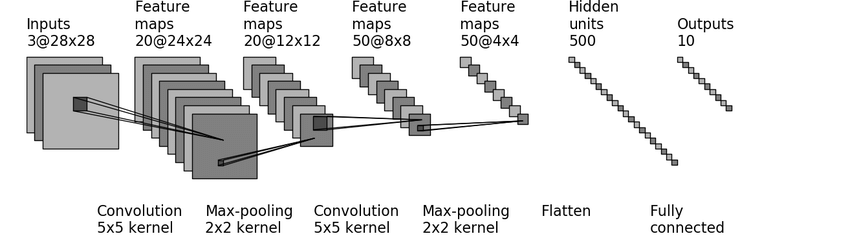
\includegraphics[width=0.9\textwidth]{figure/Lenet-5.png}
    \caption{Lenet-5 网络架构}
    \label{fig3-1}
\end{figure}

\subsubsection{本次实验使用的网络}

这次我搭建的网络基于Lenet-5,并在其之上调整了一些层,并修改了一些参数,代码采用类似pytorch风格搭建网络

\begin{lstlisting}
net = Sequential(
    Conv2d(1, 24, 5, 1, 0), ReLU(),
    MaxPool2d(2, 2, 0),
    Conv2d(24, 60, 5, 1, 0), ReLU(),
    MaxPool2d(2, 2, 0),
    Flatten(),
    Linear(60*4*4, 240), Dropout(0.8), ReLU(),
    Linear(240, 84), Dropout(0.8), ReLU(),
    Linear(84, 10)
)
\end{lstlisting}

对比Lenet网络,我对层的输入通道数,全连接层的feature数进行了一些调整,并从Sigmoid函数激活改为ReLU函数激活。

第一次训练后发现模型因为被我改复杂了,在MNIST(本实验数据集)上有过拟合的情况,训练集准确度可达到99.9\%,但验证集不到98\%,所以后期实现并加入了Dropout层,保留概率0.8,训练结果见下一章。

\subsection{模型训练}

\subsubsection{小批量随机梯度下降}

随机梯度下降(SGD)是一种常用的训练优化算法,每次更新使用一个样本计算梯度。优点是每次更新计算量小,但梯度估计噪声大,收敛不稳定。通过将训练集升一个维度,一次训练多个样本便演化为小批量随机梯度下降,小批量随机梯度下降的基本步骤如下:

\begin{enumerate}
    \item \textbf{初始化模型参数}:随机初始化模型参数。
    \item \textbf{划分小批量}:将训练数据集划分为多个小批量(使用Dataloader),每个小批量包含若干样本,小批量随机从训练集中取出。
    \item \textbf{循环更新参数}:
    \begin{enumerate}
        \item 从训练数据集中随机抽取一个小批量样本。
        \item 计算小批量样本的损失函数对模型参数的梯度。
        \item 更新模型参数:
        $$
            \theta = \theta - \eta L(\theta) 
        $$
        其中,$\theta$ 是模型参数,$\eta$ 是学习率,$L(\theta)$ 是损失函数。
\end{enumerate}
    \item 重复步骤3,直到满足停止条件,在这里是达到一定的训练轮数(epochs)。
\end{enumerate}

\subsubsection{学习率衰减}

在训练过程中学习率是一个很重要的超参数,太大会导致模型参数震荡不收敛,太小会减慢收敛速度,浪费训练时间,训练过程可以理解为一个逐步向最优点逼近的过程,所以学习率可以先大后小,这就是学习率衰减(Learning rate decay),在pytorch中一般使用lr\_scheduler进行管理,在这里直接在train函数中手动衰减。

\subsubsection{实际模型训练}

设置超参数批量大小128,学习率0.001,每迭代10轮学习率乘以0.4,训练轮数25进行训练。

\subsection{K邻近算法}

为了与CNN进行对比,我同时也写了一个简单的K邻近算法(KNN),KNN的原理非常直观:给定一个未知类别的数据点,它的类别由距离其最近的 K 个已知类别的数据点来决定,如果一个样本在特征空间中与已知类别的样本非常接近,那么它很有可能属于这个类别。

从上面可以知道,KNN需要一个超参数K,在确定K时需要慎重选择。较小的K值会增加模型的复杂度,使其对噪声敏感,而较大的K值可能会使得模型过于简单,忽略了数据内部的细节。在这里由于篇幅限制,不展开介绍,仅在最后分析模型结果。

\section{实验环境与平台}

本次试验的硬件信息如下\ref{table3-1},在我的个人笔记本上进行训练,表格,包括设备信息,设备配置等。

\begin{table}[h]
    \caption{\textbf{硬件信息}}
    \label{table3-1}
    \centering
    \begin{tabularx}{\linewidth}{>{\centering}p{3.4cm} >{\centering\arraybackslash}X}
        \toprule 
        \textbf{项目}   &   \textbf{信息} \\
        \midrule
        设备名称     &   82RC Legion Y7000P IAH7 \\
        CPU         &   12th Gen Intel i7-12700H (20) @ 4.600GHz \\
        GPU         &   NVIDIA Corporation GA107BM [GeForce RTX 3050 Ti Mobile] \\
        RAM         &   16GB \\
        系统类型     &   x86\_64 \\
        \bottomrule
    \end{tabularx}
\end{table}

\vspace*{2cm}

实验机系统在linux,表格\ref{table3-2}包括系统信息,版本信息等。

\begin{table}[h]
    \caption{\textbf{软件信息}}
    \label{table3-2}
    \centering
    \begin{tabularx}{\linewidth}{>{\centering}p{3.4cm} >{\centering\arraybackslash}X}
        \toprule 
        \textbf{项目}       &   \textbf{信息} \\
        \midrule 
        操作系统类型         &   Arch Linux x86\_64 \\
        系统版本            &  6.9.1-arch1-1 \\
        cuda版本            &   12.4 \\
        python版本          &   3.11.7 \\
        numpy版本           &   1.26.3 \\
        pytorch版本         &   2.20(cuda ver.) \\
        scikit\_learn版本    &   1.4.2 \\
        \bottomrule
    \end{tabularx}
\end{table}




\section{结果与分析}

\subsection{模型预测结果分析}

对于CNN,训练过程的可视化数据如\ref{fig4-1}所示,该网络在MNIST训练集下在第一个epoch就可以收敛地不错,之后训练集准确度保持在0.990左右,验证集准确度在0.987左右,基本符合CNN训练MNIST训练集的情况。

\begin{figure}[h!]
    \centering
    \includesvg[width=0.7\textwidth]{figure/train.svg}
    \caption{训练中损失,训练集准确度和验证集准确度}
    \label{fig4-1}
\end{figure}

对于CNN预测分类的混淆矩阵如\ref{fig4-2},从矩阵中分析,发现CNN网络对于‘5’、‘6’、‘9’的识别能力稍差,总体来看识别比较准确。

\begin{figure}[h!]
    \centering
    \includesvg[width=0.55\textwidth]{figure/confuse.svg}
    \caption{混淆矩阵}
    \label{fig4-2}
\end{figure}

对于KNN和CNN两个模型,准确度,召回率,F1值的表格如下\ref{table4-1},可以看到,在各个评判标准下,KNN的都略逊色于CNN网络,这是因为CNN卷积的特性非常适合拿来做图像处理,且模型复杂,表达能力更强。

\begin{table}[h]
    \caption{\textbf{准确度,召回率,F1值}}
    \label{table4-1}
    \centering
    \begin{tabularx}{\linewidth}{XXXXX}
        \toprule 
        \textbf{模型}       &   \textbf{准确度}     & \textbf{召回率}   &   \textbf{F1} \\
        \midrule 
        CNN           &   98.864\%     &   98.859\%    &    98.858\% \\
        KNN           &   94.952\%     &   94.925\%    &    94.921\% \\
        \bottomrule
    \end{tabularx}
\end{table}

\subsection{与现有模型对比}

我在kaggle上分别上传了CNN、KNN和预训练的Resnet50模型训练后的预测,成绩如图\ref{fig4-3}所示,submission1, 2, 3分别对应ResNet50, CNN, KNN的预测成绩。

\begin{figure}[h!]
    \centering
    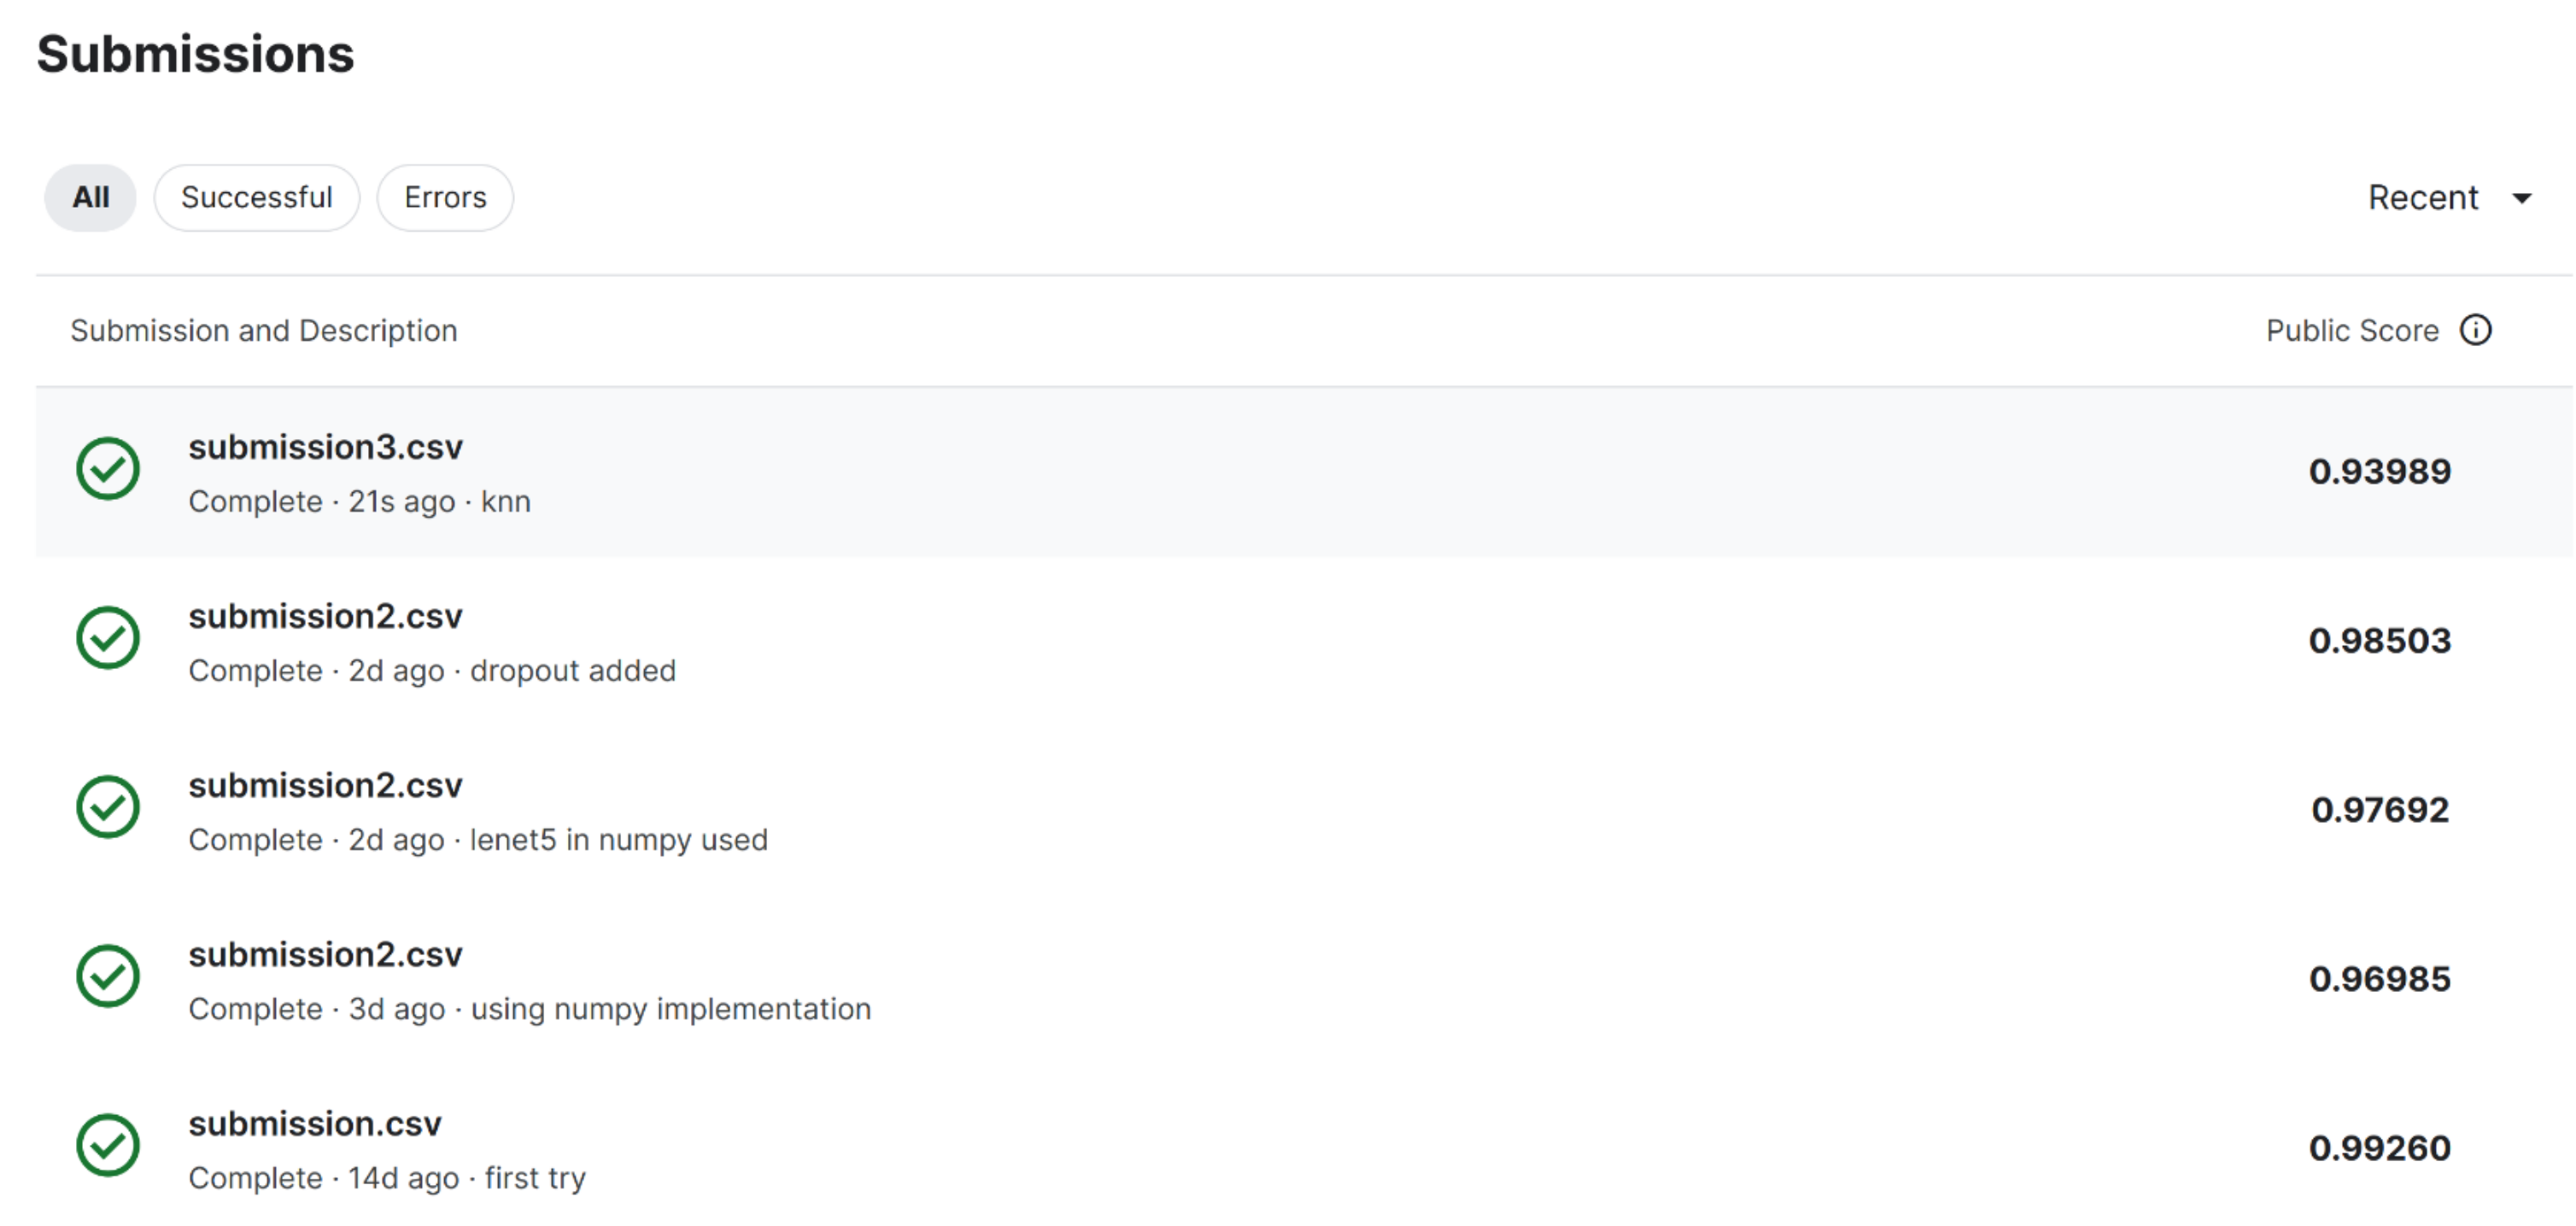
\includegraphics[width=0.7\textwidth]{figure/kaggle.png}
    \caption{kaggle分数}
    \label{fig4-3}
\end{figure}

可以看到Resnet作为深度卷积神经网络,在没有大量调参的情况下依然比其余两个numpy实现的模型效果要好上不少,而CNN也是卷积神经网络,结果比KNN要好。当然由于KNN网络的性质,如果训练得当可以在kaggle上做到全对,accuracy达到1。

\subsection{优化方向}

对于CNN网络,现有的优化方向有几条,可以改进优化器,使用Adam优化器进行梯度下降,也可以加深神经网络,采用使用新的层例如BN层(batch normalization),使用块(VGG),进行预训练等方法。

\section{个人体会}

通过机器学习这门课和这个实验,我对机器学习这个目前热门的大方向有了一个系统性的认识。在过去我因为其他的课程也略微接触到了AI领域的技术,所以在刚接触这个实验的时候,我对于深度学习的任务步骤还是有一个初步的认识,对MNIST, kaggle, CNN等名词比较熟悉,这也让我能够顺利跨过实验的初期。

但是在使用numpy手动实现CNN网络的时候,我发现我对于机器学习实践的细节还是不够熟悉,对于全连接层,卷积层等的前向和反向传播的过程一知半解,遇到了很多困难,好在最后通过查阅文献,阅读pytorch代码等方法,逐渐解决了一个个问题。

在整个模型实现后,我开始逐步调参,从最开始准确度只有不到96,发现模型的反向传播梯度有问题,到尝试使用深度神经网络,却因为使用CPU模型训练太慢而放弃,最后转头选择Lenet-5这个卷积神经网络的开山鼻祖,通过自己的探索和调参取得了不错的结果。

回头来看这次实验,还有很多做得不足的地方可以改进,对于模型,由于最后发现有一些过拟合的现象,我通过添加Dropout来减缓问题,但是其实还以通过旋转,裁剪等方法进行数据集增强,通过这来提高模型的泛化能力。

通过这个实验,我从零开始使用numpy实现了卷积神经网络和一个K邻近算法,然后和我已经很熟悉的预训练模型ResNet50进行对比,让我对与机器学习和神经网络有了一个更加全面的认识,我也锻炼了自己的编程技能和实际问题解决能力,这都让我受益良多。

%============= 参考文献 =====================
% \begin{thebibliography}{99}  


% \bibitem{ref1} 周志华. 机器学习:第3章. 清华大学出版社, 2016.







% \end{thebibliography}

\addcontentsline{toc}{section}{参考文献}
\bibliographystyle{ieeetr}
\bibliography{bible}
\clearpage
%=============  致谢  ======================

\end{document}
%%%%%%%%%% 结束 %%%%%%%%%%